\chapter{SED}\label{appendix:SED_fits}

\begin{figure}
    \centering
    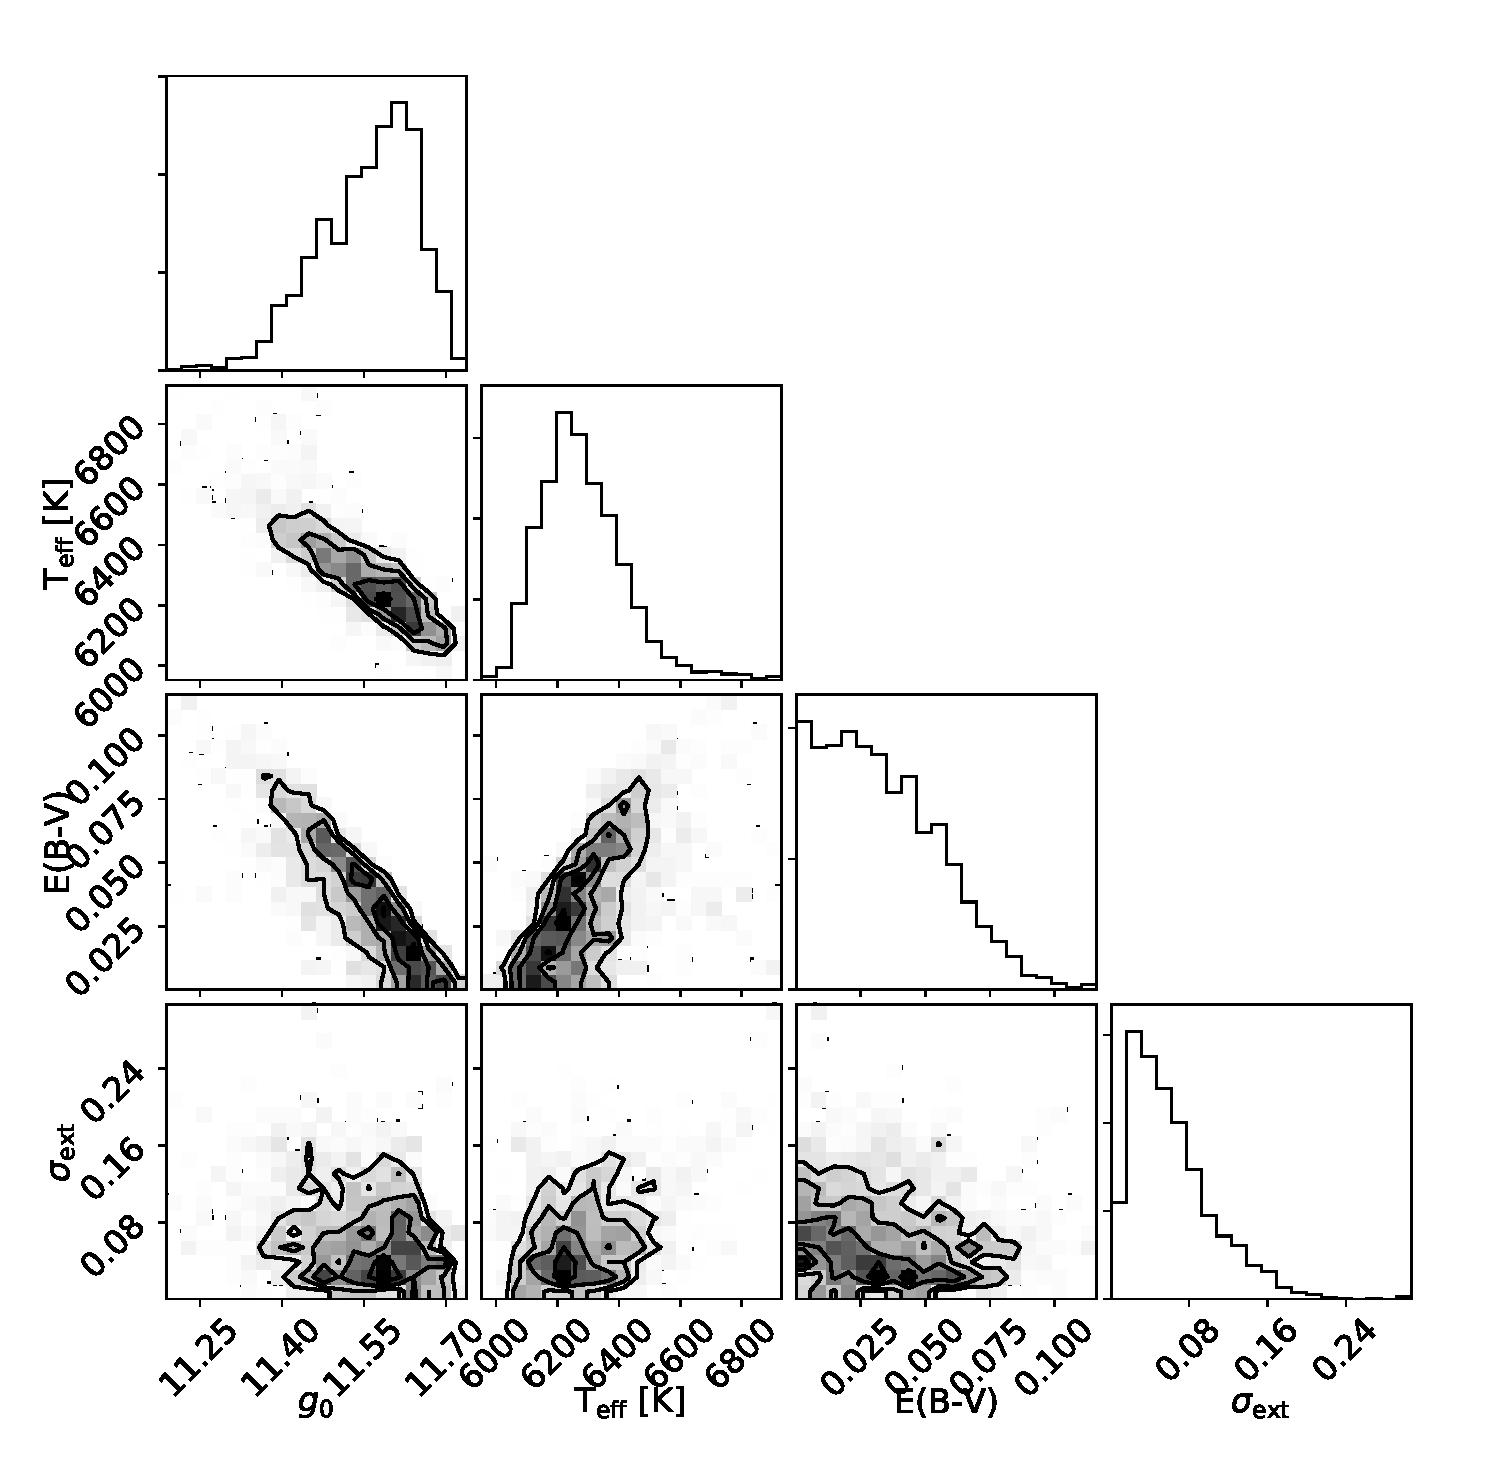
\includegraphics[scale=0.5]{Appendix/SED_fits/J2308-46.eps}
    \caption{The posterior probability distribution of EBLM J2308$-$46 from photometric fitting. Over-plotted are the 68\%, 95\% and 99.7\% contours.}
    \label{appendix:fig:SED_J2308-46}
\end{figure}

\begin{figure}
    \centering
    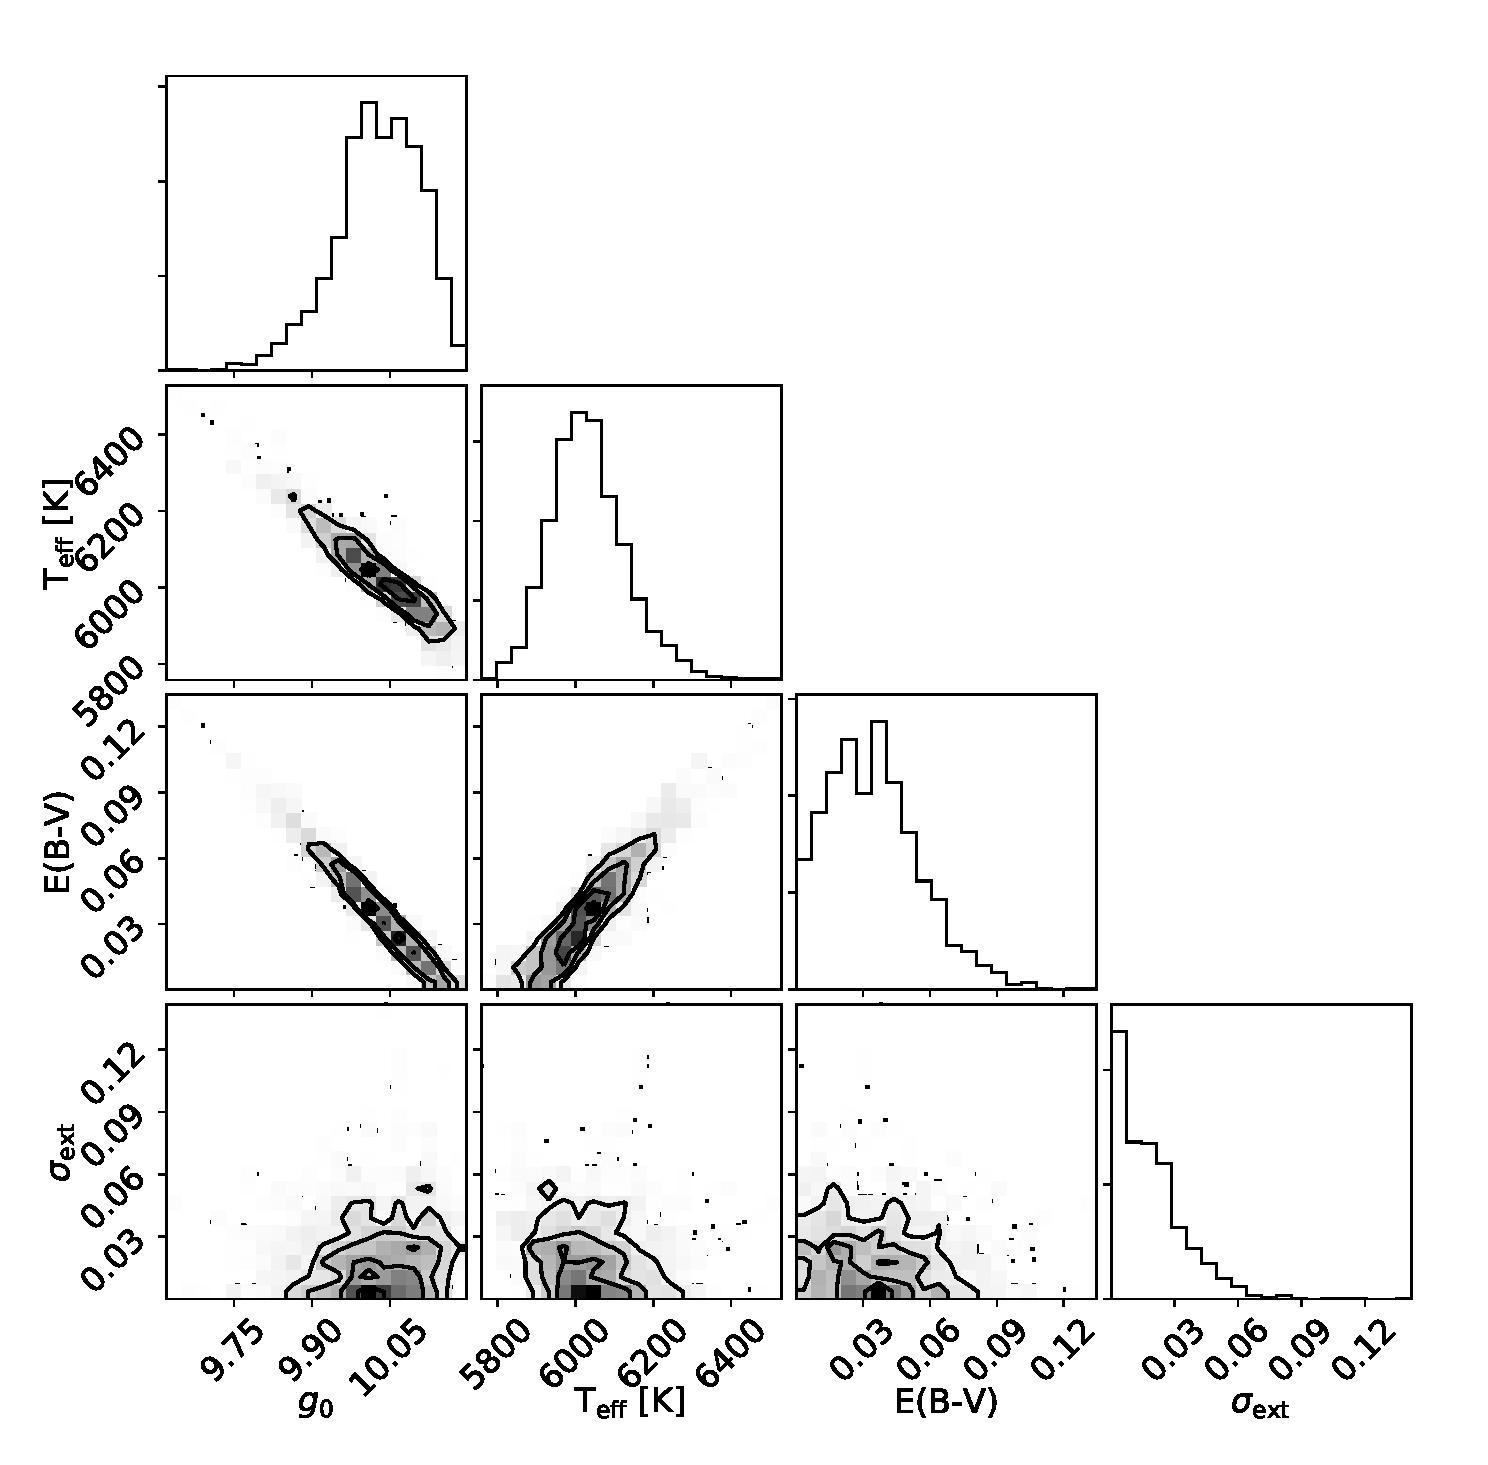
\includegraphics[scale=0.5]{Appendix/SED_fits/J0218-31.eps}
    \caption{The posterior probability distribution of EBLM J0218$-$31 from photometric fitting. Over-plotted are the 68\%, 95\% and 99.7\% contours.}
    \label{methods:fig:SED_J0218-31}
\end{figure}

\begin{figure}
    \centering
    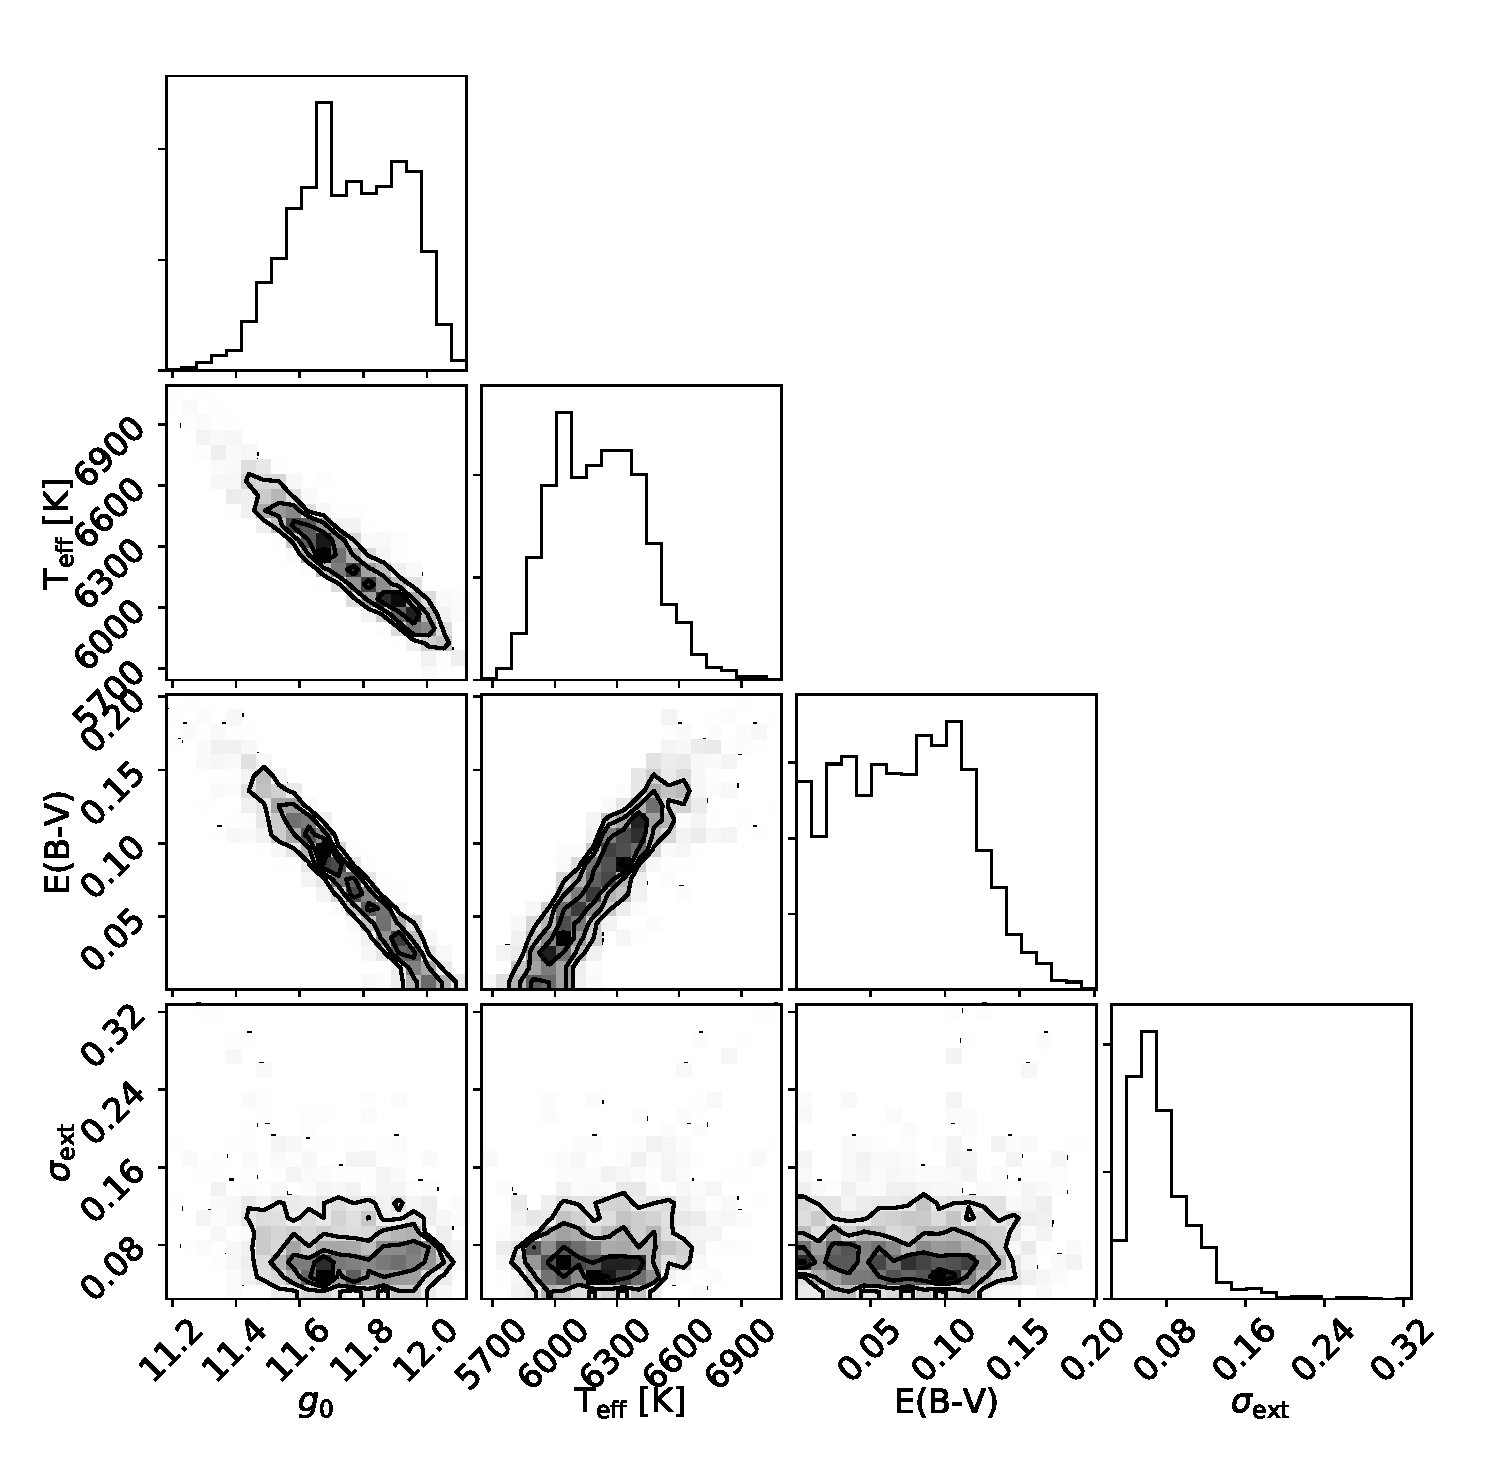
\includegraphics[scale=0.5]{Appendix/SED_fits/J1847+39.eps}
    \caption{The posterior probability distribution of EBLM J1847$+$39 from photometric fitting. Over-plotted are the 68\%, 95\% and 99.7\% contours.}
    \label{methods:fig:SED_J1847+39}
\end{figure}

\begin{figure}
    \centering
    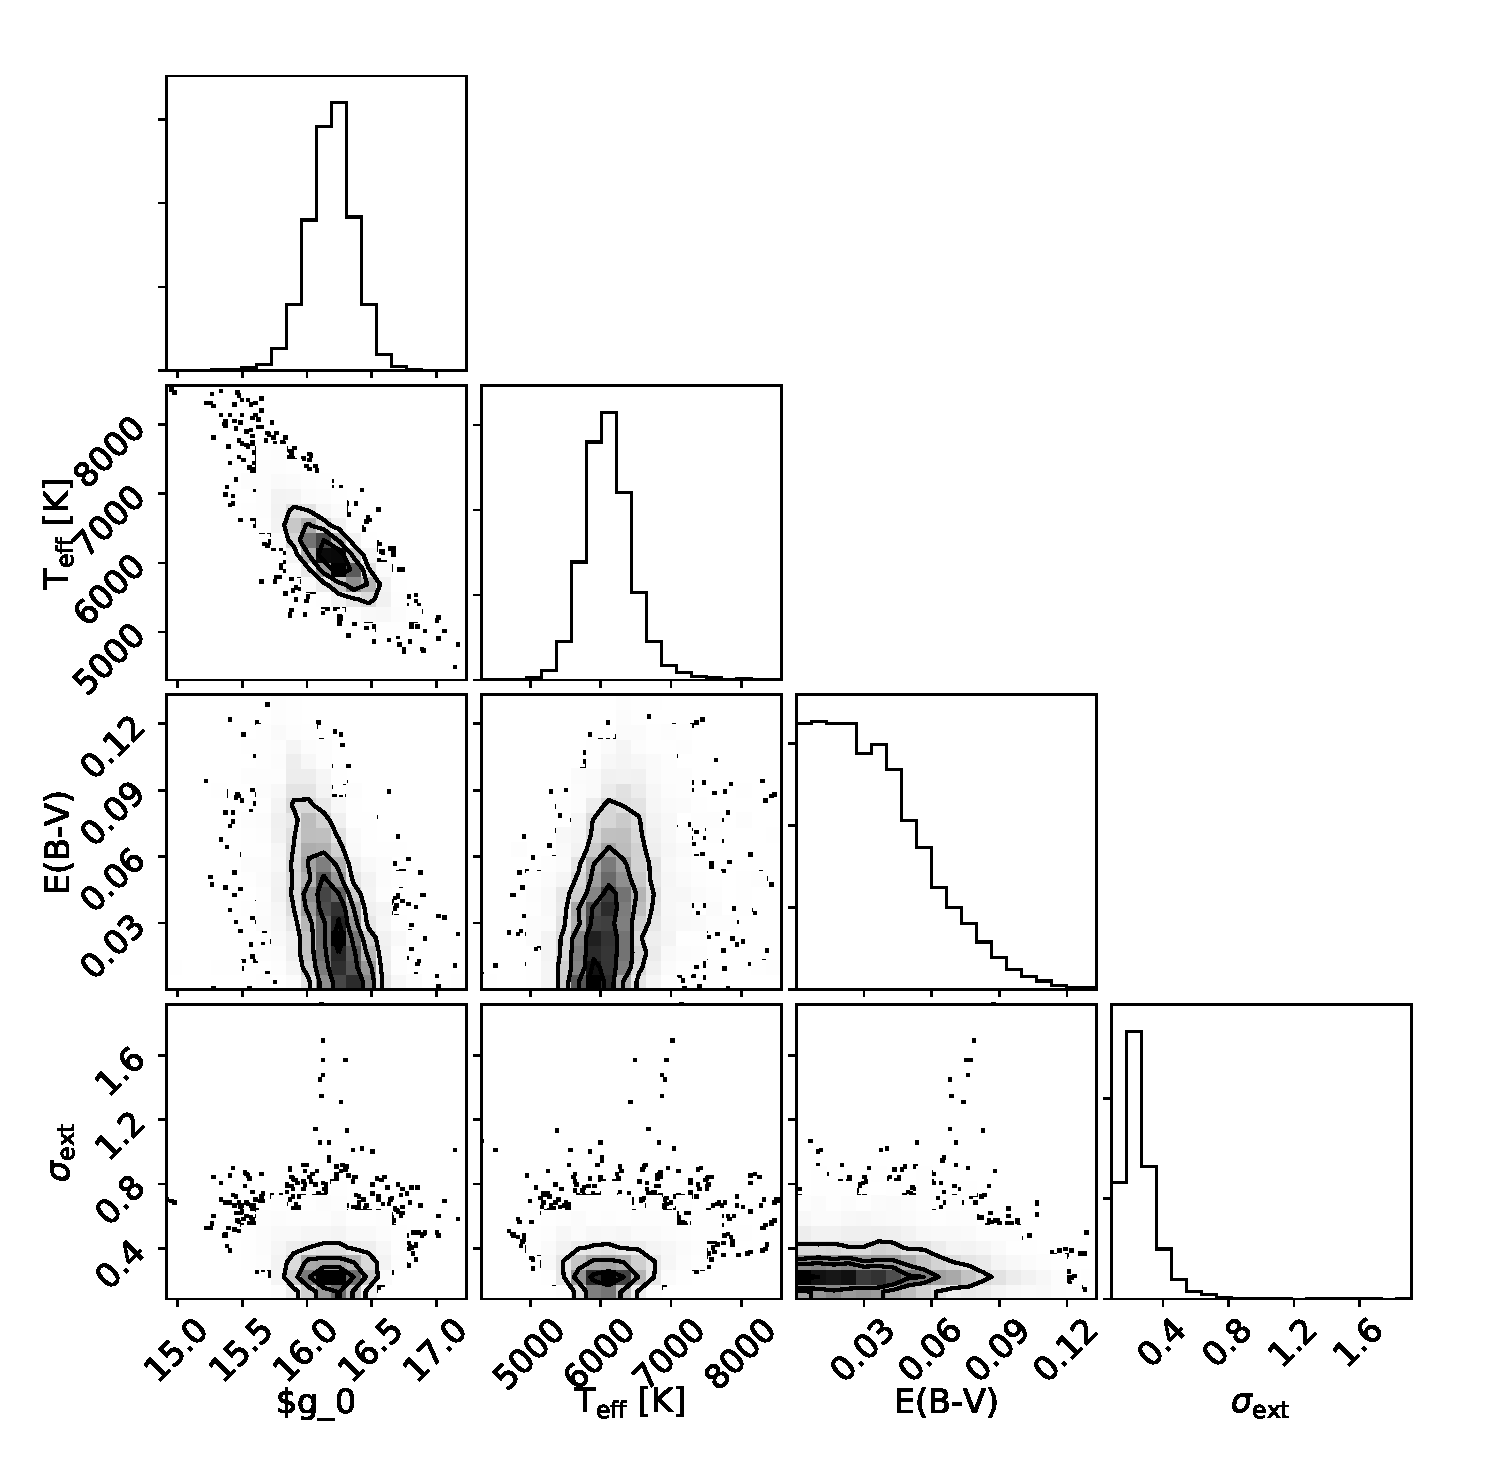
\includegraphics[scale=0.5]{Appendix/SED_fits/J1436-13.eps}
    \caption{The posterior probability distribution of EBLM J1436$-$13 from photometric fitting. Over-plotted are the 68\%, 95\% and 99.7\% contours.}
    \label{methods:fig:SED_J1436-13}
\end{figure}

\begin{figure}
    \centering
    \includegraphics[scale=0.5]{Appendix/SED_fits/J0055-00.png}
    \caption{The posterior probability distribution of EBLM J0055$-$00 from photometric fitting. Over-plotted are the 68\%, 95\% and 99.7\% contours.}
    \label{methods:fig:SED_J0055-00}
\end{figure}

\begin{figure}
    \centering
    \includegraphics[scale=0.5]{Appendix/SED_fits/J0457+14.png}
    \caption{The posterior probability distribution of EBLM J0457$+$14 from photometric fitting. Over-plotted are the 68\%, 95\% and 99.7\% contours.}
    \label{methods:fig:SED_J0457+14}
\end{figure}

\begin{figure}
    \centering
    \includegraphics[scale=0.5]{Appendix/SED_fits/J1652-19.png}
    \caption{The posterior probability distribution of EBLM J1652$-$19 from photometric fitting. Over-plotted are the 68\%, 95\% and 99.7\% contours.}
    \label{methods:fig:SED_J1652-19}
\end{figure}

\begin{figure}
    \centering
    \includegraphics[scale=0.5]{Appendix/SED_fits/J2217-04.png}
    \caption{The posterior probability distribution of EBLM J2217$-$04 from photometric fitting. Over-plotted are the 68\%, 95\% and 99.7\% contours.}
    \label{methods:fig:SED_J2217-04}
\end{figure}

\begin{figure}
    \centering
    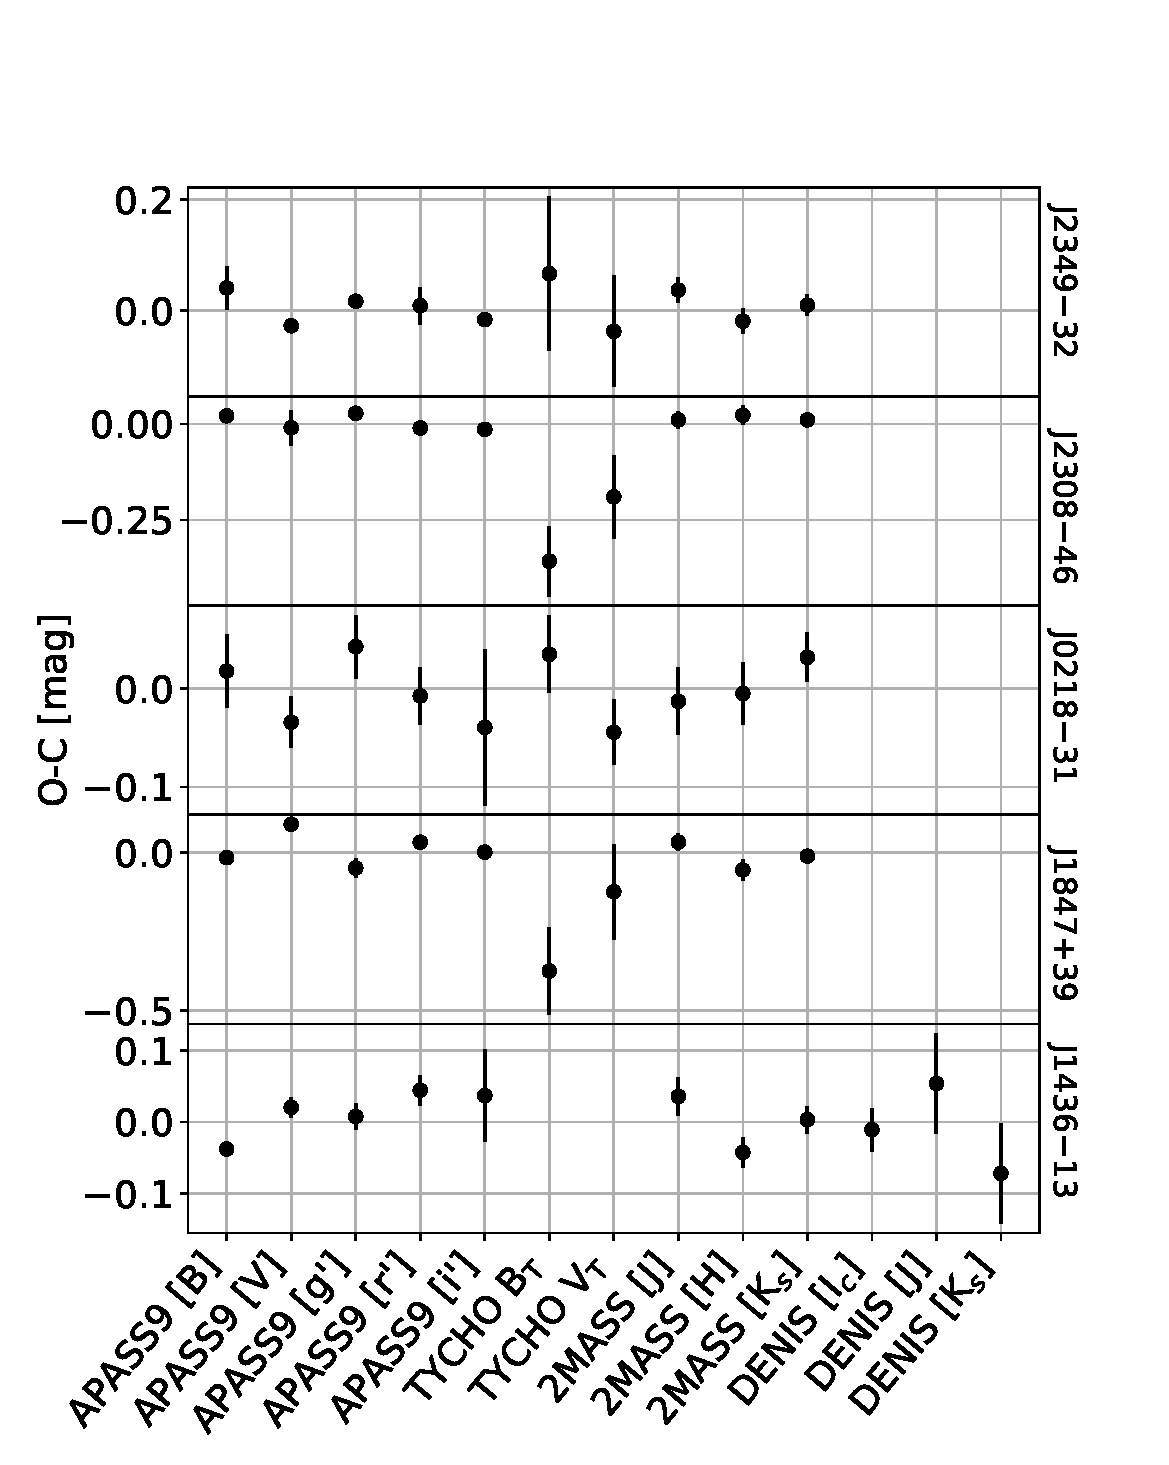
\includegraphics[scale=0.5]{Appendix/SED_fits/SED_residuals_K2.eps}
    \caption{Difference between observed and fitted magnitudes for EBLMs observed with ground-based follow-up photometry.}
    \label{fig:SED_residuals_ground}
\end{figure}

\begin{figure}
    \centering
    \includegraphics[scale=0.5]{Appendix/SED_fits/SED_residuals_ground.png}
    \caption{Difference between observed and fitted magnitudes for EBLMs observed with K2 photometry.}
    \label{fig:SED_residuals_K2}
\end{figure}